\documentclass[tikz,border=8pt]{standalone}
\usepackage{amsmath,amssymb}
\usetikzlibrary{calc,decorations.pathreplacing,positioning}

\definecolor{prepcolor}{RGB}{223,151,43}
\definecolor{qaoacolor}{RGB}{15,190,102}
\definecolor{meascolor}{RGB}{77,93,177}
\definecolor{postcolor}{RGB}{232,236,245}
\definecolor{wirecolor}{RGB}{95,95,95}
\definecolor{ctrlcolor}{RGB}{11,126,92}

\begin{document}
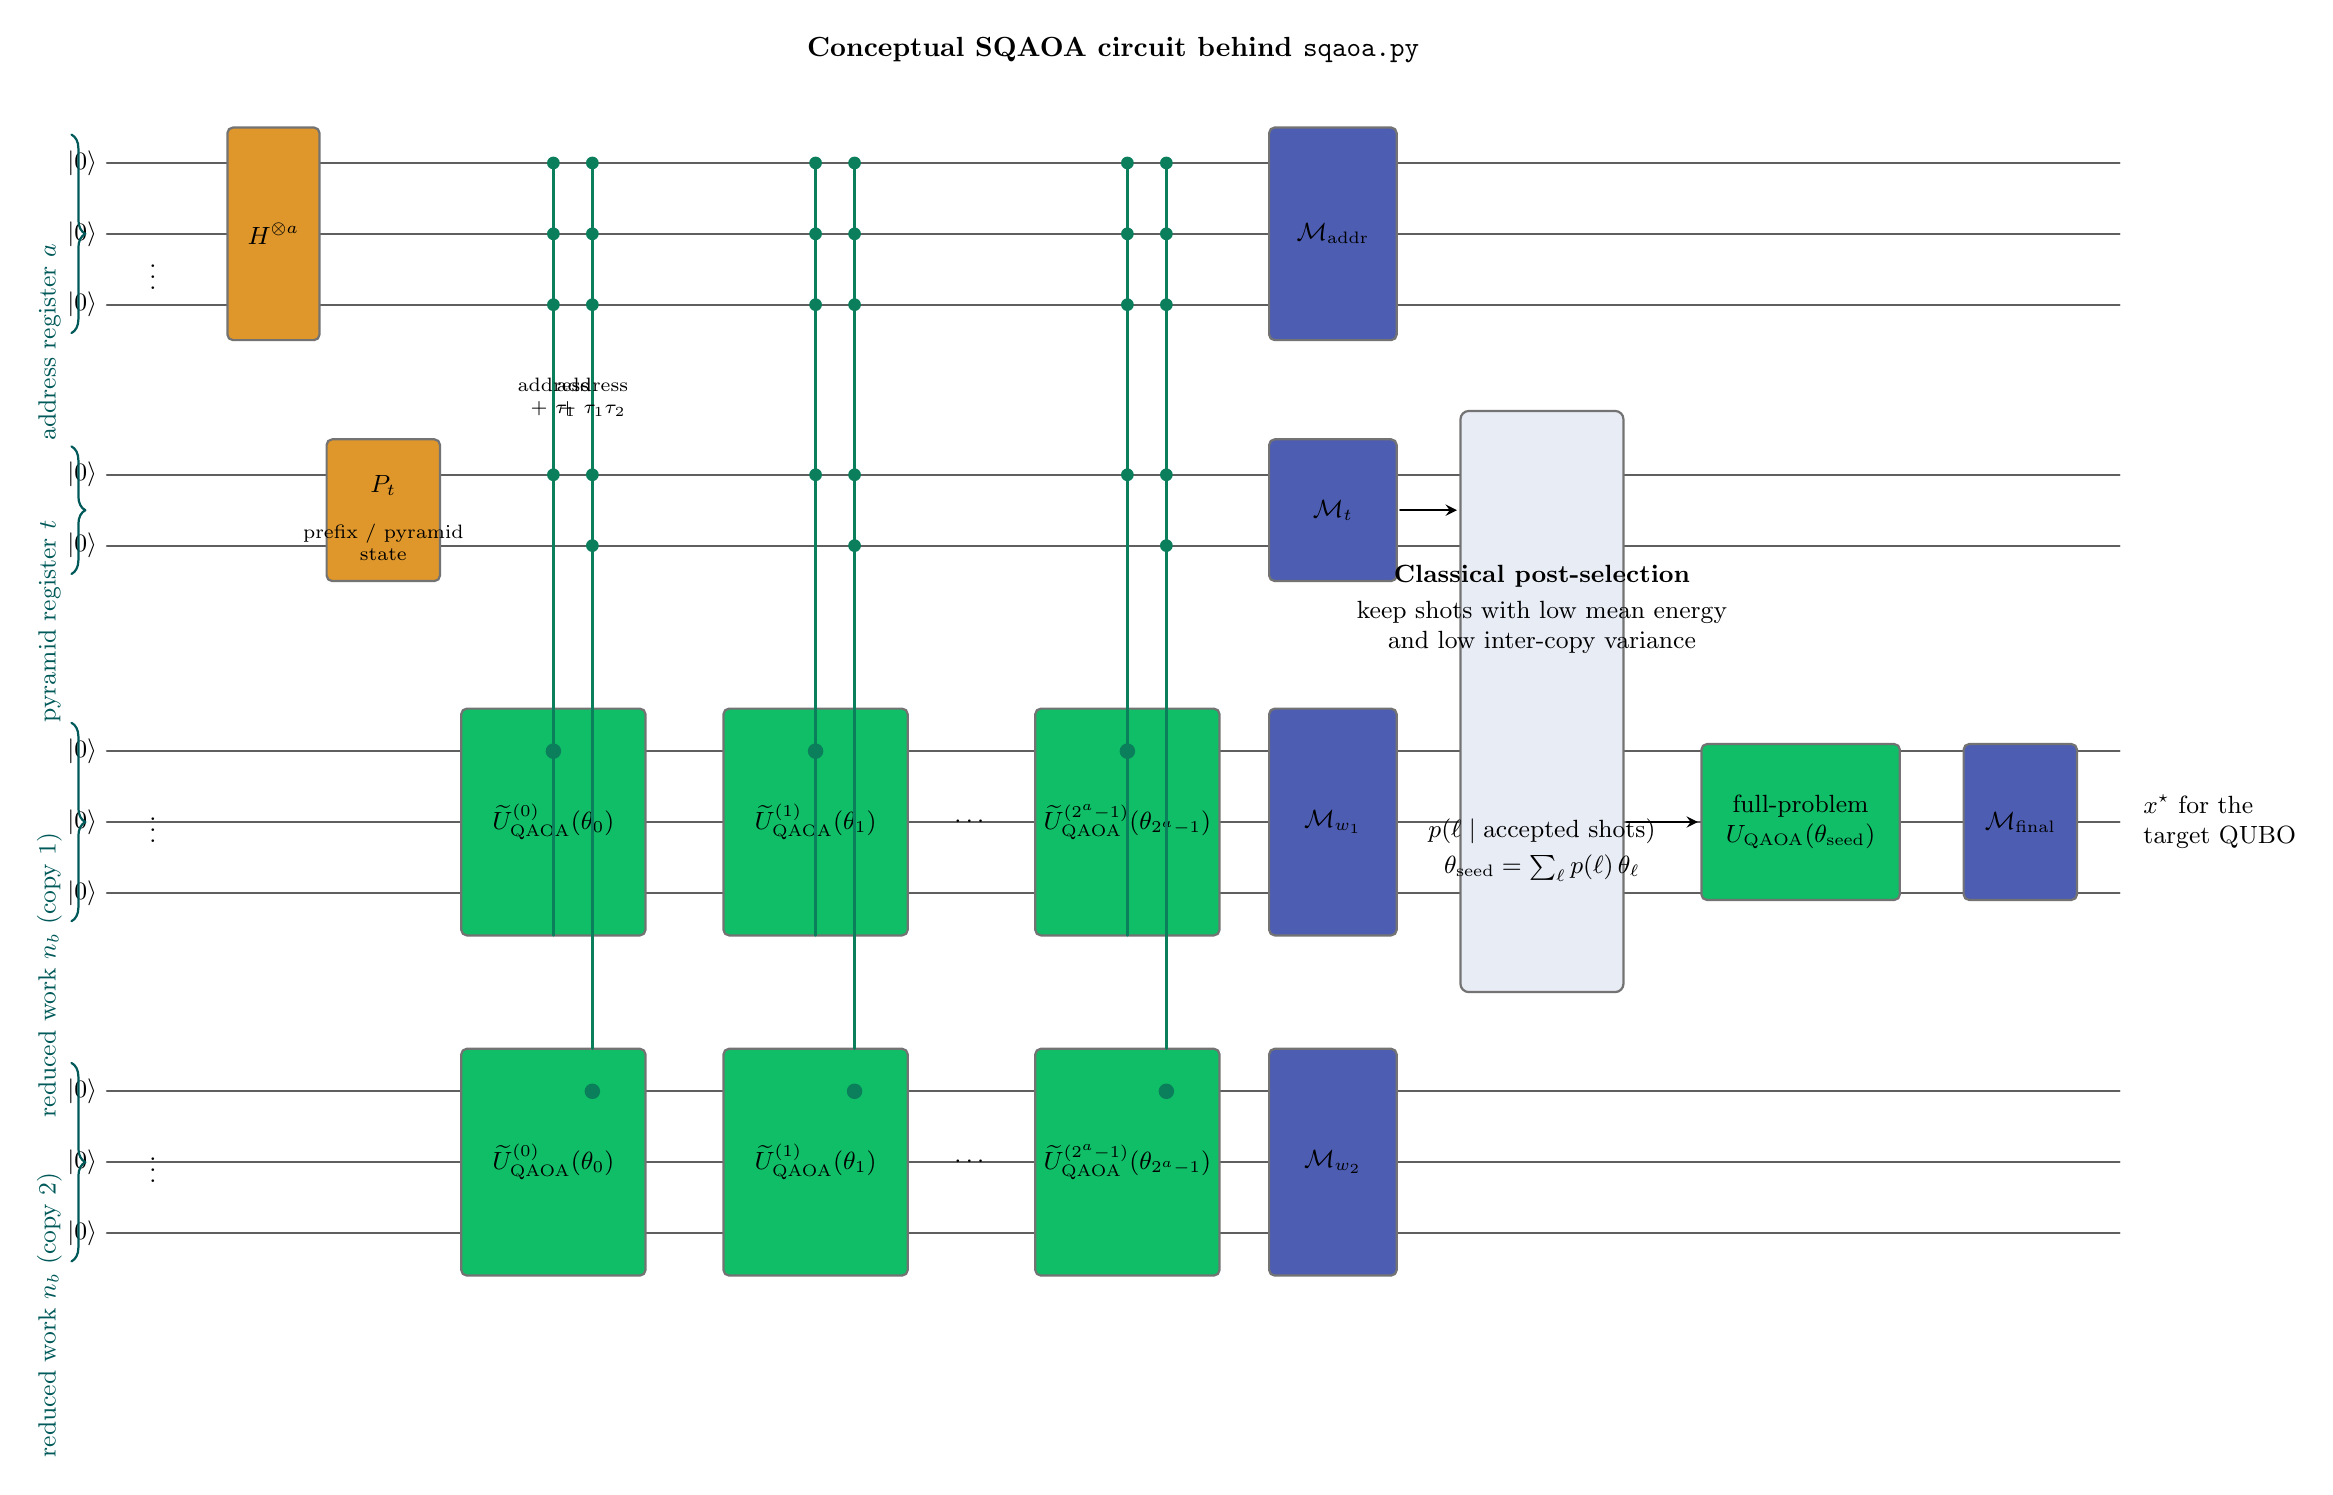
\begin{tikzpicture}[
    x=0.9cm,
    y=0.9cm,
    line cap=round,
    line join=round,
    >=stealth,
    font=\small
]

% Representative wire locations for each register block.
\def\xstart{0}
\def\xprepA{2.2}
\def\xprepT{3.8}
\def\xuone{6.3}
\def\xutwo{10.0}
\def\xuthree{14.4}
\def\xmone{17.3}
\def\xpost{20.2}
\def\xfull{23.8}
\def\xmfinal{27.0}
\def\xend{28.4}

\foreach \y in {11.5,10.5,9.5,7.1,6.1,3.2,2.2,1.2,-1.6,-2.6,-3.6} {
  \draw[wirecolor, line width=0.8pt] (\xstart,\y) -- (\xend,\y);
}

% Ket labels
\node[left] at (\xstart,11.5) {$\lvert 0\rangle$};
\node[left] at (\xstart,10.5) {$\lvert 0\rangle$};
\node[left] at (\xstart,9.5) {$\lvert 0\rangle$};
\node[left] at (\xstart,7.1) {$\lvert 0\rangle$};
\node[left] at (\xstart,6.1) {$\lvert 0\rangle$};
\node[left] at (\xstart,3.2) {$\lvert 0\rangle$};
\node[left] at (\xstart,2.2) {$\lvert 0\rangle$};
\node[left] at (\xstart,1.2) {$\lvert 0\rangle$};
\node[left] at (\xstart,-1.6) {$\lvert 0\rangle$};
\node[left] at (\xstart,-2.6) {$\lvert 0\rangle$};
\node[left] at (\xstart,-3.6) {$\lvert 0\rangle$};

% Ellipses inside grouped registers
\node at (0.65,10.0) {$\vdots$};
\node at (0.65,2.2) {$\vdots$};
\node at (0.65,-2.6) {$\vdots$};

% Left braces
\draw[decorate, decoration={brace, amplitude=5pt}, teal!70!black, line width=0.8pt]
  (-0.5,11.9) -- (-0.5,9.1)
  node[midway, left=8pt, rotate=90] {address register $a$};

\draw[decorate, decoration={brace, amplitude=5pt}, teal!70!black, line width=0.8pt]
  (-0.5,7.5) -- (-0.5,5.7)
  node[midway, left=8pt, rotate=90] {pyramid register $t$};

\draw[decorate, decoration={brace, amplitude=5pt}, teal!70!black, line width=0.8pt]
  (-0.5,3.6) -- (-0.5,0.8)
  node[midway, left=8pt, rotate=90] {reduced work $n_b$ (copy 1)};

\draw[decorate, decoration={brace, amplitude=5pt}, teal!70!black, line width=0.8pt]
  (-0.5,-1.2) -- (-0.5,-4.0)
  node[midway, left=8pt, rotate=90] {reduced work $n_b$ (copy 2)};

% Preparation blocks
\draw[rounded corners=2pt, fill=prepcolor, draw=black!55, line width=0.8pt]
  (1.7,9.0) rectangle (3.0,12.0);
\node at (2.35,10.5) {$H^{\otimes a}$};

\draw[rounded corners=2pt, fill=prepcolor, draw=black!55, line width=0.8pt]
  (3.1,5.6) rectangle (4.7,7.6);
\node at (3.9,6.95) {$P_t$};
\node[align=center, font=\scriptsize] at (3.9,6.15)
  {prefix / pyramid\\state};

% Adviser bank boxes
\foreach \x/\lab in {
  \xuone/{\widetilde U^{(0)}_{\mathrm{QAOA}}(\theta_0)},
  \xutwo/{\widetilde U^{(1)}_{\mathrm{QAOA}}(\theta_1)},
  \xuthree/{\widetilde U^{(2^a-1)}_{\mathrm{QAOA}}(\theta_{2^a-1})}
} {
  \draw[rounded corners=2pt, fill=qaoacolor, draw=black!55, line width=0.8pt]
    (\x-1.3,0.6) rectangle (\x+1.3,3.8);
  \draw[rounded corners=2pt, fill=qaoacolor, draw=black!55, line width=0.8pt]
    (\x-1.3,-4.2) rectangle (\x+1.3,-1.0);
  \node[align=center] at (\x,2.2) {$\lab$};
  \node[align=center] at (\x,-2.6) {$\lab$};
}

\node at (12.2,2.2) {$\cdots$};
\node at (12.2,-2.6) {$\cdots$};

% Measurement blocks for coherent adviser run
\draw[rounded corners=2pt, fill=meascolor, draw=black!55, line width=0.8pt]
  (16.4,9.0) rectangle (18.2,12.0);
\node[align=center] at (17.3,10.5) {$\mathcal M_{\text{addr}}$};

\draw[rounded corners=2pt, fill=meascolor, draw=black!55, line width=0.8pt]
  (16.4,5.6) rectangle (18.2,7.6);
\node[align=center] at (17.3,6.6) {$\mathcal M_t$};

\draw[rounded corners=2pt, fill=meascolor, draw=black!55, line width=0.8pt]
  (16.4,0.6) rectangle (18.2,3.8);
\node[align=center] at (17.3,2.2) {$\mathcal M_{w_1}$};

\draw[rounded corners=2pt, fill=meascolor, draw=black!55, line width=0.8pt]
  (16.4,-4.2) rectangle (18.2,-1.0);
\node[align=center] at (17.3,-2.6) {$\mathcal M_{w_2}$};

% Classical post-selection stage
\draw[rounded corners=3pt, fill=postcolor, draw=black!55, line width=0.8pt]
  (19.1,-0.2) rectangle (21.4,8.0);
\node[align=center] at (20.25,5.2)
  {\textbf{Classical post-selection}\\[2pt]
   keep shots with low mean energy\\
   and low inter-copy variance};
\node[align=center] at (20.25,1.8)
  {$p(\ell \mid \text{accepted shots})$\\[2pt]
   $\theta_{\mathrm{seed}}=\sum_{\ell}p(\ell)\,\theta_\ell$};

% Final seeded full-problem QAOA
\draw[rounded corners=2pt, fill=qaoacolor, draw=black!55, line width=0.8pt]
  (22.5,1.1) rectangle (25.3,3.3);
\node[align=center] at (23.9,2.2)
  {full-problem\\$U_{\mathrm{QAOA}}(\theta_{\mathrm{seed}})$};

\draw[rounded corners=2pt, fill=meascolor, draw=black!55, line width=0.8pt]
  (26.2,1.1) rectangle (27.8,3.3);
\node[align=center] at (27.0,2.2) {$\mathcal M_{\text{final}}$};

% Final output text
\node[align=left, anchor=west] at (28.6,2.2)
  {$x^\star$ for the\\target QUBO};

% Control columns for adviser slot 0
\foreach \y in {11.5,10.5,9.5,7.1} {
  \fill[ctrlcolor] (\xuone,\y) circle (2.3pt);
}
\draw[ctrlcolor, line width=0.9pt] (\xuone,11.5) -- (\xuone,0.6);
\fill[ctrlcolor] (\xuone,3.2) circle (2.8pt);
\node[font=\scriptsize, align=center] at (\xuone,8.2) {address\\+\ $\tau_1$};

\foreach \y in {11.5,10.5,9.5,7.1,6.1} {
  \fill[ctrlcolor] (\xuone+0.55,\y) circle (2.3pt);
}
\draw[ctrlcolor, line width=0.9pt] (\xuone+0.55,11.5) -- (\xuone+0.55,-1.0);
\fill[ctrlcolor] (\xuone+0.55,-1.6) circle (2.8pt);
\node[font=\scriptsize, align=center] at (\xuone+0.55,8.2) {address\\+\ $\tau_1\tau_2$};

% Control columns for adviser slot 1
\foreach \y in {11.5,10.5,9.5,7.1} {
  \fill[ctrlcolor] (\xutwo,\y) circle (2.3pt);
}
\draw[ctrlcolor, line width=0.9pt] (\xutwo,11.5) -- (\xutwo,0.6);
\fill[ctrlcolor] (\xutwo,3.2) circle (2.8pt);

\foreach \y in {11.5,10.5,9.5,7.1,6.1} {
  \fill[ctrlcolor] (\xutwo+0.55,\y) circle (2.3pt);
}
\draw[ctrlcolor, line width=0.9pt] (\xutwo+0.55,11.5) -- (\xutwo+0.55,-1.0);
\fill[ctrlcolor] (\xutwo+0.55,-1.6) circle (2.8pt);

% Control columns for last adviser slot
\foreach \y in {11.5,10.5,9.5,7.1} {
  \fill[ctrlcolor] (\xuthree,\y) circle (2.3pt);
}
\draw[ctrlcolor, line width=0.9pt] (\xuthree,11.5) -- (\xuthree,0.6);
\fill[ctrlcolor] (\xuthree,3.2) circle (2.8pt);

\foreach \y in {11.5,10.5,9.5,7.1,6.1} {
  \fill[ctrlcolor] (\xuthree+0.55,\y) circle (2.3pt);
}
\draw[ctrlcolor, line width=0.9pt] (\xuthree+0.55,11.5) -- (\xuthree+0.55,-1.0);
\fill[ctrlcolor] (\xuthree+0.55,-1.6) circle (2.8pt);

% A couple of short arrows to emphasize the classical flow.
\draw[->, thick] (18.25,6.6) -- (19.05,6.6);
\draw[->, thick] (21.45,2.2) -- (22.45,2.2);

% Explanatory title
\node[font=\normalsize\bfseries] at (14.2,13.1)
  {Conceptual SQAOA circuit behind \texttt{sqaoa.py}};

\end{tikzpicture}
\end{document}
